\chapter{Functions of Many Variables}
\label{ch:multivariable}

If you’ve ever hiked, you have probably seen a topographical map. Figure \ref{fig:4-1-topo} shows part of a topographic map of Stowe, Vermont.

\begin{figure}[!ht]
  \centering
    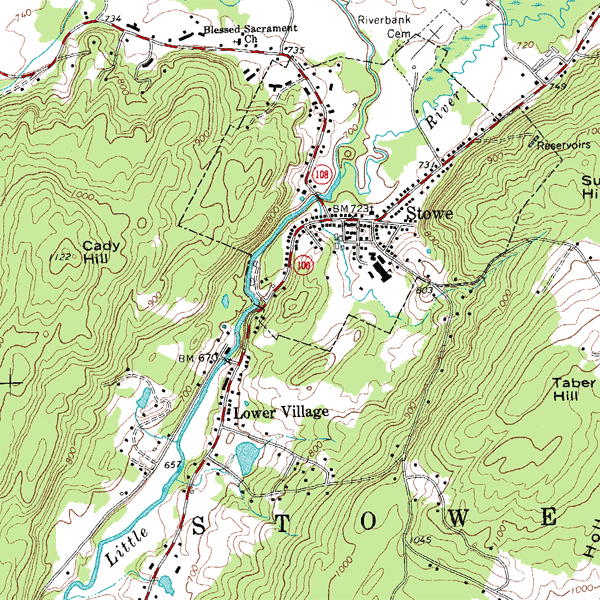
\includegraphics[width=0.4\textwidth]{img/chap4/image001.png}
    \caption{Topographical map of Stowe, VT: USGS, \url{http://en.wikipedia.org/wiki/File:Topographic_map_example.png.}}
    \label{fig:4-1-topo}
\end{figure}

Points with the same elevation are connected with curves, so you can read not only your east-west and your north-south location, but also your elevation. You may have also seen weather maps that use the same principle -- points with the same temperature are connected with curves (isotherms), or points with the same atmospheric pressure are connected with curves (isobars). These maps let you read not only a place's location but also its temperature or atmospheric pressure.

In this chapter, we will use that same idea to make graphs of functions of two variables.

%\section{Examples of Functions of Multiple Variables}
\label{sec:examples}

\subsection{Pre-Calculus Idea -- Topological Maps}
If you’ve ever hiked, you have probably seen a topographical map. Figure \ref{fig:4-1-topo} shows part of a topographic map of Stowe, Vermont.

\begin{figure}[!ht]
  \centering
    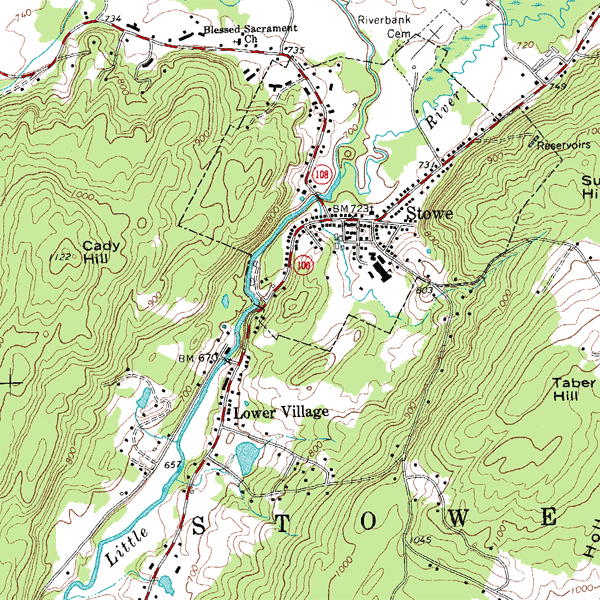
\includegraphics[width=0.4\textwidth]{img/chap4/image001.png}
    \caption{Topographical map of Stowe, VT: USGS, \url{http://en.wikipedia.org/wiki/File:Topographic_map_example.png.}}
    \label{fig:4-1-topo}
\end{figure}

Points with the same elevation are connected with curves, so you can read not only your east-west and your north-south location, but also your elevation. You may have also seen weather maps that use the same principle -- points with the same temperature are connected with curves (isotherms), or points with the same atmospheric pressure are connected with curves (isobars). These maps let you read not only a place's location but also its temperature or atmospheric pressure.

In this chapter, we will use that same idea to make graphs of functions of two variables.

\section{Multivariable Functions}
\label{sec:multivariable-functions}

\subsection{Introduction}
Real life is rarely as simple as one input / one output. Many relationships depend on lots of variables. Here are some examples.
\begin{itemize}
  \item If I put a deposit into an interest-bearing account and let it sit, the amount I have at the end of three years depends on $P$ (how much my initial deposit is), $r$ (the annual interest rate), and $n$ (the number of compoundings per year).

  \item The air resistance on a wing in a wind tunnel depends on the shape of the wing, the speed of the wind, the wing's orientation (pitch, yaw, and roll), plus a myriad of other things that I can't begin to describe.

  \item The amount of your television cable bill depends on which basic rate structure you have chosen and how many pay-per-view movies you ordered.
\end{itemize}
Since the real world is so complicated, we want to extend our calculus ideas to functions of several variables.

\subsection{Functions of Two Variables}
If $x_1, x_2, x_3,\ldots, x_n$ are real numbers, then $(x_1,x_2,x_3,\ldots, x_n)$ is called an {\bf $n$-tuple}. This is an extension of ordered pairs and triples. A function of $n$ variables is a function whose domain\index{Domain} is some set of $n$-tuples and whose range\index{Range} is some set of real numbers.

For much of what we do here, everything will work the same whether we were working with 2, 3, or 47 variables. Because we're trying to keep things a little bit simpler, we'll concentrate on functions of two variables.

\begin{definition}[A Function of Two Variables]
A {\bf function of two variables}\index{Function}\index{Function!of two variables} is a function, that is, to each input is associated exactly one output.
    \begin{itemize}
    \item The inputs are ordered pairs, $(x,y)$. 
    \item The outputs are real numbers (each output is a single real number). 
    \item The domain of a function is the set of all possible inputs (ordered pairs); 
    \item the range is the set of all possible outputs (real numbers).
    \item The function can be written $z=f(x,y)$.
    \end{itemize}
Functions of two variables can be described numerically (a table), graphically, algebraically (a formula), or in English.
\end{definition}
We will often now call the familiar $y=f(x)$ a {\bf function of one variable}\index{Function!of one variable}.

\begin{example}
The cost of renting a car depends on how many days you keep it and how far you drive. Represent this using a function.

\begin{solution} Let $d$ be the number of days you rent the car, and $m$ be the number of miles you drive. Then the cost of the car rental $C(d,m)$ is a function of two variables.
\end{solution}\end{example}

\begin{example}
The demand for hot dog buns depends on the price for the hot dog buns and also on the price for hot dogs. Represent this as a function.

\begin{solution} The demand $q_B=f(p_B,p_D)$ is a function of two variables. (The demand for hot dogs also depends on the price of both dogs and buns).
\end{solution}\end{example}

\subsection{Formulas and Tables}
Just as in the case of functions of one variable, we can display a function of two variables in a table. The two inputs are shown in the margin (top row, left column), and the outputs are shown in the interior cells.

\begin{example}
Table \ref{tab:4-1-rentcar} shows the cost $C(d,m)$ in dollars to rent a car for $d$ days and drive it $m$ miles.

\begin{table}[ht!]
\centering
    \begin{tabular}{*{5}{c}}
    $d$ & \multicolumn{4}{c}{$m$} \\
    \toprule
        & 100 & 200 & 300 & 400\\
    \midrule
    1   &  55 &  70 &  85 & 100\\	
    2   &  95 & 110 & 125 & 140\\	
    3   & 135 & 150 & 165 & 180\\
    \bottomrule
    \end{tabular}
    \caption{Cost, in dollars, to rent a car for $d$ days and drive $m$ miles.}
    \label{tab:4-1-rentcar}
\end{table}
\begin{enumerate}[label=(\alph*)]
    \item What is the cost to rent a car for 3 days and drive it 200 miles?

    \begin{solution} 
    According to the table, renting the car for three days (row with $d=3$) and driving it 200 miles (column with $m=200$) will cost \$150.
    \end{solution}
    \item What is $C(100,4)$? What is $C(4,100)$?

    \begin{solution} 
    Careful now -- the input is an ordered pair, so in $C(100,4)$, the 100 has to be a value of $d$ and the 4 has to be a value of $m$, so $C(100,4)$ would be the cost of renting a car for 100 days and driving it 4 miles. That cost is not in the table. (And that would be a pretty silly way to rent a car.) On the other hand, $C(4,100)$ is the cost of renting for 4 days and driving 100 miles. The table says that would cost \$175.
    \end{solution}
    \item Suppose we rent the car for three days. Is $C$ an increasing function with $d$ fixed at 3?

    \begin{solution} 
If we know that $d$ is fixed at 3, we're looking at $C(3,m)$. This is now a function of one variable: just $m$. We can see the table that displays values of this function by focusing our attention on just the row where $d=3$.
\begin{table}[ht!]
\centering
    \begin{tabular}{*{5}{c}}
    $d$ & \multicolumn{4}{c}{$m$} \\
    \toprule
        & 100 & 200 & 300 & 400\\
    \midrule
    3   & 135 & 150 & 165 & 180\\
    \bottomrule
    \end{tabular}
\end{table}
Now we can see that if we rent for 3 days, the cost appears to be an increasing function of the number of miles we drive, which shouldn't be surprising.
    \end{solution}
\end{enumerate}
\end{example}

The idea of fixing one variable and watching what happens to the function as the other varies will come up again and again.

It's hard to display a function of more than two variables in a table. But it's convenient to work with formulas for functions of two variables, or as many variables as you like.

\begin{example}
The cost $C(d,m)$ in dollars to rent a car for $d$ days and drive it $m$ miles is given by the formula
$$C(d,m)=40d+0.15m \enspace .$$

\begin{enumerate}[label=(\alph*)]
    \item What is the cost of renting a car for 3 days and driving it 200 miles?

    \begin{solution}
     $C(3,200) = 40(3)+0.15(200)=\$150$. This is the same value we got from the table. The formula will give us the same answers for any of the table values.
    \end{solution}
    \item What is $C(100,4)$? What is $C(4,100)$?

    \begin{solution}
    $C(100,4)$ makes perfect sense to the formula (even if it doesn't make sense for actually renting a car). So now we can get an answer. To rent the car for 100 days and drive it for 4 miles should cost \$4000.60. $C(4,100)=\$175$, as before.
    \end{solution}
    \item Suppose we rent the car for three days. Is $C$ an increasing function with $d$ fixed at 3?

    \begin{solution}
    If we fix $d=3$, then $C(d,m)$ becomes $C(3,m)=40(3)+0.15m=120+0.15m$. Yes, this is an increasing function of $m$ -- we can tell because it's linear and its slope is $0.15>0$.
    \end{solution}
\end{enumerate}
\end{example}

Reality check -- the formula that gives the cost for the rental car makes sense for all values of $d$ and $m$. But that's not how the real cost works -- you can't rent the car for a negative number of days or drive a negative number of miles. (That is, there are domain restrictions.) In addition, most car rental agreements don't compute a charge for fractions of days; they round up to the next whole number of days.

\begin{example}
Let $f(x,y,z,w)=35x^2w-\frac{1}{z}+yz^2$. Evaluate $f(0,1,2,3)$.

\begin{solution} Remember that this is an ordered 4-tuple; make sure the numbers get substituted into the correct places.
$$f(0,1,2,3)= 35(0)^2(3)-\frac{1}{2}+(1)(2)^2 = 3.5$$
\end{solution}\end{example}

\subsection{Graphs}
The graph of a function of two variables is a surface in three-dimensional space. Let's start by looking at the 3-dimensional rectangular coordinate system, how to locate points in three dimensions, and distance between points in three dimensions.

In the 2-dimensional rectangular coordinate system we have two coordinate axes that meet at right angles at the origin, and it takes two numbers, an ordered pair $(x,y)$, to specify the rectangular coordinate location of a point in the plane (two dimensions).

2D coords
Each ordered pair $(x,y)$ specifies the location of exactly one point, and the location of each point is given by exactly one ordered pair $(x,y)$. The $x$ and $y$ values are the coordinates of the point $(x,y)$.

The situation in three dimensions is very similar. In the 3-dimensional rectangular coordinate system we have three coordinate axes that meet at right angles, and three numbers, an ordered triple $(x,y,z)$, are needed to specify the location of a point.

3D coords
Each ordered triple $(x,y,z)$ specifies the location of exactly one point, and the location of each point is given by exactly one ordered triple $(x,y,z)$. The $x$, $y$, and $z$ values are the coordinates of the point $(x,y,z)$. The figure below shows the location of the point $(4, 2, 3)$.

Point (4,2,3)
Typically we use a right-hand orientation. To see what this means, imagine your right hand in front hand in front of you with the palm toward your face, your thumb pointing up, you index finger straight out, and your next finger toward your face (and the two bottom fingers bent into the palm). Then, in the right hand coordinate system, your thumb points along the positive $z$-axis, your index finger along the positive $x$-axis, and the other finger along the positive $y$-axis.

hand
Other orientations of the axes are possible and valid (with appropriate labeling), but the right-hand system is the most common orientation and is the one we will generally use. If another orientation is used, then the axes will be explicitly labeled.

Each ordered triple $(x,y,z)$ specifies the location of a single point, and this location point can be plotted by locating the point $(x,y,0)$ on the $xy$-plane and then going up $z$ units (the red path in the figure below).

Plotting
We could also get to the same $(x,y,z)$ point in other ways. For instance, we could start by finding the point $(x,0,z)$ on the $xz$-plane and then going $y$ units parallel to the $y$-axis, or by finding $(0,y,z)$ on the $yz$-plane and then going $x$ units parallel to the $x$-axis (the blue path in the figure above).

\begin{example}
Plot the locations of the points
\begin{itemize}
    \item $P=(0,3,4)$,
    \item $Q=(2,0,4)$,
    \item $R=(1,4,0)$,
    \item $S=(3,2,1)$, and
    \item $T=(-1,2,1)$.
\end{itemize}
\begin{solution} The points are shown below.

Points
\end{solution}\end{example}

Once we can locate points, we can begin to consider the graphs of various collections of points. By the graph of $z=2$ we mean the collection of all points $(x,y,z)$ which have the form $(x,y,2)$. Since no condition is imposed on the $x$ and $y$ variables, they take all possible values. The graph of $z=2$ is a plane parallel to the $xy$-plane and 2 units above the $xy$-plane. Similarly, the graph of $y=3$ is a plane parallel to the $xz$-plane, and $x=4$ is a plane parallel to the $yz$-plane. (Note: The planes have been drawn as rectangles, but they actually extend infinitely far.)

PlanePlanes
\paragraph*{Distance Between Points}
In two dimensions we can think of the distance between points as the length of the hypotenuse of a right triangle, and that leads to the Pythagorean formula:
$$\mbox{distance} = \sqrt{(\Delta x)^2 + (\Delta y)^2 } \enspace .$$
2D distance
In three dimensions we can also think of the distance between points as the length of the hypotenuse of a right triangle.

3D distance
In this situation the calculations may appear more complicated, but they are straightforward and the final formula is what we hope it would be given the 2-dimensional formula:
\begin{align*}
    \mbox{distance}^2   &= \mbox{base}^2 + \mbox{height}^2 \\
                        &= \left(\sqrt{(\Delta x)^2 + (\Delta y)^2}\right)^2 + (\Delta z)^2\\
                        &= (\Delta x)^2 + (\Delta y)^2 + (\Delta z)^2
\end{align*}
so
    $$\mbox{distance} = \sqrt{(\Delta x)^2 + (\Delta y)^2 + (\Delta z)^2}$$

\begin{theorem}[Distance in 3-Dimensions]
If $P=(x_1,y_1,z_1)$ and $Q=(x_2,y_2,z_2)$ are points in space, then the distance between $P$ and $Q$ is
\begin{align*}
\mbox{distance} &= \sqrt{(\Delta x)^2 + (\Delta y)^2 + (\Delta z)^2} \\
                &= \sqrt{(x_2-x_1)^2 + (y_2-y_1)^2 + (z_2-z_1)^2}
\end{align*}
\end{theorem}

The 3-dimensional pattern is very similar to the 2-dimensional pattern with the additional piece $\Delta z)^2$.

\begin{example}
Find the distances between points $A=(1,2,3)$ and $B=(7,5,-3$).

\begin{solution}
  $$\mbox{Dist}(A,B) = \sqrt{6^2+3^2+(-6)^2} = \sqrt{36+9+36} = \sqrt{81} = 9 \enspace .$$
\end{solution}\end{example}

In two dimensions, the set of points at a fixed distance from a given point is a circle, and we used the distance formula to determine equations describing circles: the circle with center $(2, 3)$ and radius 5 is given by $(x-2)^2 + (y-3)^2 = 5^2$ or $x^2+y^2-4x-6y = 12$.

Circle
The same ideas work for spheres in three dimensions.

\begin{definition}[Sphere]
The set of points $(x,y,z)$ at a fixed distance $r$ from a point $(a,b,c)$ is a {\bf sphere} with center $(a,b,c)$ and radius $r$.

[Sphere]
The sphere is given by the equation
$$(x-a)^2+(y-b)^2+(z-c)^2=r^2 \enspace .$$
\end{definition}

\begin{example}
Write the equations of a sphere with center $(2, -3, 4)$ and radius 3.

\begin{solution} The equation is
$$(x-2)^2+(y+3)^2+(z-4)^2=3^2=9.$$
\end{solution}\end{example}

Now suppose that we want to graph a surface. We can think of each input $(x,y)$ as a location on the plane, and plot the point $f(x,y)$ units above that point. Graphing that can be challenging. We have a few options:

Use a computer program (such as GeoGebra or Mathematica) to draw beautiful perspective drawings.

Graph
If such a program is available, then this is usually the most accurate option.

Try to draw a perspective drawing by hand. This is very challenging, and usually not worth the effort.
Use level curves to draw contour diagrams (or contour maps), which is the approach we'll focus on here. A contour diagram is like a topographical map -- points with the same elevation (outputs) are connected with curves. Each particular output is called a level, and these curves are called level curves or contours. The closer the curves are to each other, the steeper that section of the surface. Topographical maps give hikers information about elevation, steep and shallow grades, peaks and valleys. Contour diagrams give us the same kind of information about a function.
Below is a contour diagram of the same surface shown in above. The level curves are graphs in the $xy$-plane of curves $f(x,y)=c$ for various constants $c$.

Contour map
Each of the squares corresponds to one of the bumps on the surface. If the contours are positive, as highlighted below, the bump is above the $xy$-plane. If the contours are negative, the bump extends below the $xy$-plane.

Contour map
Everywhere on the crisscrossed pattern of diagonal lines, the height of the surface is 0, so the surface is on the $xy$-plane. This is a feature that we wouldn't necessarily have seen when we looked at the perspective drawing. Contour maps can help us see features of the surface that the 3-dimensional graph doesn't show.

Contour map
To better understand contour diagrams, suppose we had a table of elevation data. We could graph this by plotting the height at each point and connecting the dots with smooth curves, which would result in the something like the graph shown.

TableSurface
If we slice the surface above with the plane $z=8$, the points where the plane cuts the surface are those points where the elevation of the surface is 8 units above the $xy$-plane. The figure below shows the surface being sliced by the planes $z=8$ and $z=4$. Slicing the surface at different elevations and sketching the curves where the plane intersects the surface results in the second graph below.

SlicesLevel curves
If we move all of those curves to the $xy$-plane (or, equivalently, view them from directly overhead), the result is a 2-dimensional graph of the level curves of the original surface. This is the contour diagram.

Contour map
\begin{example}
Create a contour diagram for our car rental example with cost function $C(d,m)=40d+0.15m$. Draw curves for when the cost is 0, 100, 200, 300, and 400.

\begin{solution}
  We'll set $C(d,m)=40d+0.15m=c$ for $c = 0, 100, 200, 300$, and 400 and draw the curves in the $dm$-plane.

The first coordinate of the ordered pair is $d$, so the $d$-axis will be horizontal; the $m$-axis will be vertical. Remember that the domain for this function is really just where $d \geq 0$ and $m \geq 0$, so we will only draw the curves in the first quadrant.

When $c=0$:
\begin{align*}
C(d,m)  &= 40d + 0.15m = 0 \\
0.15m   &= -40d \\
m       &= \frac{40}{0.15}d \approx   -267d
\end{align*}
This is the equation of a line, with slope about $-267$, passing through the origin. Because of the domain restrictions, the curve we will draw for this level is simply the origin. Putting this back into the car rental context, the only point where we pay \$0 for renting the car is when we rent the car for 0 days and drive it 0 miles -- that is, if we don't rent it at all.

When $c=100$:
\begin{align*}
C(d,m) = 40d + 0.15m &= 100 \\
    0.15m &= -40d+100 \\
    m &= -\frac{40}{0.15}d + \frac{100}{0.15}\approx   -267d+667
\end{align*}
This is the equation of a line, with slope about $-267$, and $d$-intercept of about 667. This section of this line that lies in the first quadrant is shown with 100 labeling it.

Putting this into context, any point on that line represents a $(d,m)$ combination of days and miles that will make the cost exactly \$100. So, for example -- if we rent the car for 0 days and drive it 667 miles, it will cost us \$100. If we rent the car for 2.5 days and don't drive it at all, it will cost us \$100.

We continue for $c= 200, 300$, and 400 and sketch the curves in the plane, resulting in the contour diagram shown to the right.

Contour map
\end{solution}\end{example}

\begin{example}
The contour diagram for the cost $C(d,m)$ in dollars for renting a car for d days and driving it m miles is shown in the previous example. Use the diagram to answer the following questions.
\begin{enumerate}[label=(\alph*)]
    \item What is the cost of renting a car for 3 days and driving it 200 miles?

    \begin{solution} The point $(3, 200)$ is between contours on this graph, so we can’t get an exact answer for $C(3,200)$. (But it’s typical for a graph that we would have to estimate). It looks to me as if $(3, 200)$ is halfway between the 100 and the 200 contours, so let's estimate that $C(3,200)$ is about \$150.

Estimates from the graph are necessarily very rough. The graph only shows a little information (in this way, a contour diagram is like a table), so we have to extrapolate in between. But for most graphs, we don’t actually know what happens between the contours. All we know for sure is that the output at $(3, 200)$ is between the two levels we see. For this car rental example, we also know a formula, and my table showed this particular input, so we have other ways to get a better answer.
    \end{solution}
    \item What is $C(100,4)$? What is $C(4,100)$?

    \begin{solution} We can't find $(100, 4)$ on this diagram, so we can't make an estimate of $C(100,4)$ from this graph. $(4, 100)$ lies between the contours for 100 and 200. It looks closer to 200, so let's estimate that $C(4,100)$ is about \$180.
    \end{solution}
    \item Suppose we rent the car for 3 days. Is $C$ an increasing function of miles?

    \begin{solution} If we fix $d=3$, we get a vertical line. What happens as $m$ increases on this vertical line? As $m$ increases, the function values shown on the contours increase, so $C$ appears to be an increasing function of miles.
    \end{solution}
\end{enumerate}
Contour map
\end{example}

\begin{example}
Here is a contour diagram for a function $g(x,y)$.

Contour map
Use the diagram to answer the following questions:

What is $g(3,5)$?
What is the highest point shown on the diagram? What is the lowest point shown?
If you start at $(3, 5)$ and head in the positive $x$ direction, do you go uphill or downhill first?

\begin{solution}
$g(3,5)$ is 0.6. We can tell because the point is right on one of the contours, as illustrated in the image below.

Contour with points
The highest contour shown is 0.9, and there would be a contour for 1.0 if the surface had ever got that high. However, the height seems to be increasing as we move in toward the center, so it appears that g gets to nearly 1 in the center. The lowest contour is 0.1. But again, we will guess that the height continues to decrease, so it appears that $g$ is nearly 0 around the outside.
Starting at the point $(3, 5, 0.6)$ on the surface and traveling to the right along the horizontal line shown in the previous part, we would cross the contour for 0.7 next. So the function increases first (we go uphill), and then decreases again.
Again, remember that we don't really know what happens between the contours. All we can do is estimate from the information in the graph.
\end{solution}\end{example}

\begin{example}
Here is a contour diagram for a function $F(x,y)$.

Contour map
Describe the shape of the surface.
Suppose you travel along the surface in the positive $y$-direction, starting on the surface at the point above (or below) the point $(x,y)=(-1,1)$. Describe your journey.

\begin{solution}
  The surface is bumpy, with regularly spaced oval bumps. Notice that some of the bumps go up (positive contours), but others go down. Between the bumps, there are horizontal lines that are completely level, with an elevation of 0.
It looks as if $F(-1,1)$ is about 3. As we head in the positive y-direction along the line shown below, we first go uphill, nearly to 4, then we start going downhill. As we keep going north, we keep descending, going into the dip, until nearly $-4$. We're starting to go uphill again just as we leave the graph.

Contour map
\end{solution}\end{example}

What happens if you have a function of more than two variables? Its graph will be a hyper-surface. For example, the graph of a function of four variables will be a hyper-surface in 5-dimensional space. This is very difficult (impossible for most of us) to visualize. Even the contours are hard to visualize -- instead of curves in the plane, they’re hyper-surfaces in 4-dimensional space. So if you have more than two variables, the graph isn't usually very useful.

%Functions of Two Real-Life Variables
\subsection{Complementary Goods and Substitute Goods}
The demand for some pairs of goods have a relationship, where the quantity demanded for one product depends somehow on the prices for both
\begin{definition}[Complementary Goods]
Two goods are {\bf complementary}\index{complimentary goods} if an increase in the price of either decreases the demand for both.
\end{definition}

\begin{example}
\begin{itemize}
  \item The demand for cars depends on both the price for cars and the price of gasoline.
  \item The demand for hot dog buns depends on both the price for the buns and the price for the hot dogs.
\end{itemize}
\end{example}

\begin{definition}[Substitute Goods]
Two goods are {\bf substitutes} if an increase in the price of one increases the demand for the other.
\end{definition}

\begin{example}
\begin{itemize}
  \item The demand for Brand A depends on its price and also on the price of its main competitor Brand B. If the Brand B raises its price, consumers will switch brands (substitute) and demand for Brand A will increase.
\end{itemize}
\end{example}
Think about brands of soft drinks, detergent, or paper towels. A traditional example is coffee and tea: the idea is that consumers are simply looking for a hot drink and they'll buy whatever is cheaper. But this has always seemed fishy to me -- I've never met any coffee- or tea-drinkers who would happily switch.

These demand functions are functions of two variables.

\begin{example}
The demand functions for two products are given below. $p_1$, $p_2$, $q_1$, and $q_2$ are the prices (in dollars) and quantities for Products 1 and 2:
\begin{align*}
q_1 &= 200-3p_1-p_2\\
q_2 &= 150-p_1-2p_2
\end{align*}
Are these two products complementary goods or substitute goods? What is the quantity demanded for each when the price for Product 1 is \$20 per item and the price for Product 2 is \$30 per item?

\begin{solution} These products are complementary: an increase in either price decreases both demands. You can see that because the coefficients are both negative in each demand function.

When $p_1=20$ and $p_2=30$, we have
\begin{align*}
q_1 &= 200-3(20)-(30)=110\\ 
q_2 &= 150-(20)-2(30)=70
\end{align*}
So 110 units are demanded for Product 1 and 70 units are demanded for Product 2 when the price for Product 1 is \$20 per item and the price for Product 2 is \$30 per item.
\end{solution}\end{example}

\subsection{Cobb-Douglas Production Function}
\label{ssec:cobb-douglas}
Production functions are used to model the total output of a firm for a variety of inputs (doesn't this sound like a function of several variables?). One example is a {\bf Cobb-Douglas Production function}\index{Cobb-Douglas Production function}:
$$P=AL^{\alpha}K^{\beta} \enspace ,$$
where $P$ is the total production, $A$ is a constant, $\alpha$ and $\beta$ are constants between 0 and 1, $L$ is the labor force, and $K$ is the capital expenditure. (The units must be massaged well.)

You can read more about Cobb-Douglas Production functions at \url{http://en.wikipedia.org/wiki/Cobb-Douglas}. You can read about other kinds of production functions at \url{http://en.wikipedia.org/wiki/Production_function}.

\section{Partial Derivatives}
\label{sec:derivatives}

Now that you have some familiarity with functions of two variables, it's time to start applying calculus to help us solve problems with them. In Chapter 2, we learned about the derivative for functions of two variables. Derivatives told us about the shape of the function, and let us find local max and min – we want to be able to do the same thing with a function of two variables.

First let's think. Imagine a surface, the graph of a function of two variables. Imagine that the surface is smooth and has some hills and some valleys. Concentrate on one point on your surface. What do we want the derivative to tell us? It ought to tell us how quickly the height of the surface changes as we move… Wait, which direction do we want to move? This is the reason that derivatives are more complicated for functions of several variables – there are so many (in fact, infinitely many) directions we could move from any point.

It turns out that our idea of fixing one variable and watching what happens to the function as the other changes is the key to extending the idea of derivatives to more than one variable.

Partial Derivatives
Partial Derivatives
Suppose that z=f(x,y) is a function of two variables.

The partial derivative of f with respect to x is the derivative of the function f(x,y) where we think of x as the only variable and act as if y is a constant.

The partial derivative of f with respect to y is the derivative of the function f(x,y) where we think of y as the only variable and act as if x is a constant.

The with respect to x or with respect to y part is really important – you have to know and tell which variable you are thinking of as THE variable.

Geometrically
Geometrically the partial derivative with respect to x gives the slope of the curve as you travel along a cross-section, a curve on the surface parallel to the x-axis. The partial derivative with respect to y gives the slope of the cross-section parallel to the y-axis.

Notation for the Partial Derivative
The partial derivative of z=f(x,y) with respect to x is written as
fx(x,y)
or simply
fxorzx.
The Leibniz notation is
∂f∂x
or
∂z∂x.
We use an adaptation of the ∂z∂x notation to mean find the partial derivative of f(x,y) with respect to x:
∂∂x(f(x,y))=∂f∂x
To estimate a partial derivative from a table or contour diagram
The partial derivative with respect to x can be approximated by looking at an average rate of change, or the slope of a secant line, over a very tiny interval in the x-direction (holding y constant). The tinier the interval, the closer this is to the true partial derivative.

To compute a partial derivative from a formula
If f(x,y) is given as a formula, you can find the partial derivative with respect to x algebraically by taking the ordinary derivative thinking of x as the only variable (holding y fixed).

Of course, everything here works the same way if we're trying to find the partial derivative with respect to y – just think of y as your only variable and act as if x is constant.

The idea of a partial derivative works perfectly well for a function of several variables: you focus on one variable to be THE variable and act as if all the other variables are constants.

\begin{example}
Here is a contour diagram for a function g(x,y).

Contour map
Use the diagram to answer the following questions:

Estimate gx(3,5) and gy(3,5).
Where on this diagram is gx greatest? Where is gy greatest?

\begin{solution} gx(3,5) means we're thinking of x as the only variable, so we'll hold y fixed at y=5. That means we’ll be looking along the horizontal line y=5. To estimate gx, we need two function values. (3, 5) lies on the contour line, so we know that g(3,5)=0.6. The next point as we move to the right is g(4.2,5)=0.7.

Now we can find the average rate of change:
Average rate of change ====(change in output)(change in input)ΔgΔx0.7-0.64.2-3112\approx   0.083
We can do the same thing by going to the next point we can read to the left, which is g(2.4,5)=0.5. Then the average rate of change is
ΔgΔx=0.5-0.62.4-3=16\approx   0.167.
Either of these would be a fine estimate of gx(3,5) given the information we have, or we could take their average. We can estimate that gx(3,5)\approx   0.125.

Estimate gy(3,5) the same way, but moving on the vertical line. Using the next point up, we get the average rate of change is
ΔgΔy=0.7-0.65.8-5=18=0.125.
Using the next point down, we get
ΔgΔy=0.5-0.64.5-5=15=0.2.
Taking their average, we estimate gy(3,5)\approx   0.1625.

gx means x is our only variable, and we're thinking of y as a constant. So we're thinking about moving across the diagram on horizontal lines. gx will be greatest when the contour lines are closest together, i.e., when the surface is steepest – then the denominator in ΔgΔx will be small, so ΔgΔx will be big. Scanning the graph, we can see that the contour lines are closest together when we head to the left or to the right from about (0.5, 8) and (9, 8). So gx is greatest at about (0.5, 8) and (9, 8). For gy, we want to look at vertical lines. gy is greatest at about (5, 3.8) and (5, 12).
\end{solution}\end{example}

\begin{example}
Cold temperatures feel colder when the wind is blowing. Windchill is the perceived temperature, and it depends on both the actual temperature and the wind speed – a function of two variables! You can read more about windchill at http://www.nws.noaa.gov/om/windchill/. Below is a table that shows the perceived temperature for various temperatures and windspeeds.

Windchill table
(Table courtesy of the National Weather Service, http://www.nws.noaa.gov/om/windchill/images/windchill.gif.)
Note that they also include the formula, but for this example we'll use the information in the table.

What is the perceived temperature when the actual temperature is 25°F and the wind is blowing at 15 miles per hour?
Suppose the actual temperature is 25°F. Use information from the table to describe how the perceived temperature would change if the wind speed increased from 15 miles per hour?

\begin{solution}
  Reading the table, we see that the perceived temperature is 13°F
This is a question about a partial derivative. We’re holding the temperature (T) fixed at 25°F, and asking what happens as wind speed (V) increases from 15 miles per hour. We’re thinking of V as the only variable, so we want WindChillV=WV when T=25 and V=15. We'll find the average rate of change by looking in the column where T=25 and letting V increase, and use that to approximate the partial derivative.
WV\approx   ΔWΔV=11-1320-15=-0.4
What are the units? W is measured in °F and V is measured in mph, so the units here are °F/mph. And that lets us describe what happens: The perceived temperature would decrease by about 0.4°F for each mph increase in wind speed.
\end{solution}\end{example}

\begin{example}
Find fx and fy at the points (0, 0) and (1, 1) if f(x,y)=x2-4xy+4y2.

\begin{solution}
  To find fx, take the ordinary derivative of f with respect to x, acting as if y is constant:
fx(x,y)=2x-4y.
Note that the derivative of the 4y2 term with respect to x is zero because it's a constant (as far as x is concerned).

Similarly,
fy(x,y)=-4x+8y.
Now we can evaluate these at the points:

fx(0,0)=0 and fy(0,0)=0; this tells us that the cross sections parallel to the x- and y- axes are both flat at (0,0).

fx(1,1)=-2 and fy(1,1)=4; this tells us that above the point (1, 1), the surface decreases if we move to more positive x values and increases if we move to more positive y values.
\end{solution}\end{example}

\begin{example}
Find ∂f∂x and ∂f∂y if f(x,y)=ex+yy3+y+yln(y).

\begin{solution}
  ∂f∂x means x is our only variable, we're thinking of y as a constant. Then we'll just find the ordinary derivative. From x's point of view, this is an exponential function, divided by a constant, with a constant added. The constant pulls out in front, the derivative of the exponential function is the same thing, and we need to use the chain rule, so we multiply by the derivative of that exponent (which is just 1):
∂f∂x=1y3+yex+y.
∂f∂y means that we're thinking of y as the variable, acting as if x is constant. From y's point of view, f is a quotient plus a product, so we'll need the quotient rule and the product rule:
∂f∂y==( )( )-( )( )( )2+( )( )+( )( )(ex+y(1))(y3+y)-(ex+y)(3y2+1)(y3+y)2+(1)(ln(y))+(y)(1y)
\end{solution}\end{example}

\begin{example}
Find fz if f(x,y,z,w)=35x2w-1z+yz2.

\begin{solution}
  fz means we act as if z is our only variable, so we'll act as if all the other variables (x, y, and w) are constants and take the ordinary derivative:
fz(x,y,z,w)=1z2+2yz.
\end{solution}\end{example}

Using Partial Derivatives to Estimate Function Values
We can use the partial derivatives to estimate values of a function. The geometry is similar to the tangent line approximation in one variable. Recall the one-variable case: if x is close enough to a known point a, then
f(x)\approx   f(a)+f′(a)(x-a).
In two variables, we do the same thing in both directions at once:

Approximating Function Values with Partial Derivatives
To approximate the value of f(x,y), find some point (a,b) where

(x,y) and (a,b) are close, that is, x and a are close and y and b are close.
You know the exact values of f(a,b) and both partial derivatives there.
Then
f(x,y)\approx   f(a,b)+fx(a,b)(x-a)+fy(a,b)(y-b).
Notice that the total change in f is being approximated by adding the approximate changes coming from the x and y directions. Another way to look at the same formula:
Δf\approx   fxΔx+fyΔy.
How close is close? It depends on the shape of the graph of f. In general, the closer the better.

\begin{example}
Use partial derivatives to estimate the value of f(x,y)=x2-4xy+4y2 at (0.9, 1.1).

\begin{solution}
  Note that the point (0.9, 1.1) is close to an easy point, (1, 1). In fact, we already worked out the partial derivatives at (1, 1): fx(x,y)=2x-4y so fx(1,1)=-2, and fy(x,y)=-4x+8y so fy(1,1)=4. We also know that f(1,1)=1.

So,
f(0.9,1.1)\approx   1-2(-0.1)+4(0.1)=1.6.
Note that in this example it would have been possible to simply compute the exact answer:
f(0.9,1.1)=(0.9)2-4(0.9)(1.1)+4(1.1)2=1.69.
Our estimate is not perfect, but it's pretty close.
\end{solution}\end{example}

\begin{example}
Here is a contour diagram for a function g(x,y). Use partial derivatives to estimate the value of g(3.2,4.7).

Contour map
\begin{solution}
  This is the same diagram from before, so we already estimated the value of the function and the partial derivatives at the nearby point (3,5). g(3,5) is 0.6, our estimate of gx(3,5)\approx   0.125, and our estimate of gy(3,5)\approx   0.1625. So
g(3.2,4.7)\approx   0.6+(0.125)(0.2)+(0.1625)(-0.3)=0.57625.
Note that in this example we have no way to know how close our estimate is to the actual value.
\end{solution}\end{example}

% Application: Option pricing and "the Greeks."

%\section{Optimization with Multivariable Functions}
\label{sec:multi-opt}

The partial derivatives tell us something about where a surface has local maxima and minima. Remember that even in the one-variable cases, there were critical points which were neither maxima nor minima – this is also true for functions of many variables. In fact, as you might expect, the situation is even more complicated.

\subsection{Second Derivatives}
When you find a partial derivative of a function of two variables, you get another function of two variables – you can take its partial derivatives, too. We've done this before, in the one-variable setting. In the one-variable setting, the second derivative gave information about how the graph was curved. In the two-variable setting, the second partial derivatives give some information about how the surface is curved, as you travel on cross-sections – but that's not very complete information about the entire surface.

Imagine that you have a surface that's ruffled around a point, like what happens near a button on an overstuffed sofa, or a pinched piece of fabric, or the wrinkly skin near your thumb when you make a fist. Right at that point, every direction you move, something different will happen – it might increase, decrease, curve up, curve down… A simple phrase like concave up or concave down can't describe all the things that can happen on a surface.

Surprisingly enough, though, there is still a second derivative test that can help you decide if a point is a local maximum or minimum or neither, so we still do want to find second derivatives.

\begin{definition}[Second Partial Derivatives]
Suppose $f(x,y)$ is a function of two variables. Then it has four {\bf second partial derivatives}\index{Derivative!second partial}\index{Second partial derivative}:
$$f_{xx} = \frac{\partial}{\partial x}(f_x) = (f_x)_x \quad f_{xy} = \frac{\partial}{\partial y}(f_x)=(f_x)_y $$
$$f_{yx} = \frac{\partial}{\partial x}(f_y) = (f_y)_x \quad f_{yy} = \frac{\partial}{\partial y}(f_y)=(f_y)_y \enspace .$$
$f_{xy}$ and $f_{yx}$ are called the {\bf mixed (second) partial derivatives}\index{Mixed partial derivative} of $f$.

Leibniz notation for the second partial derivatives is a bit confusing, and we won't use it as often.
$$f_{xx} = \frac{\partial}{\partial x}\left(\frac{\partial f}{\partial x}\right) = \frac{\partial^2 f}{\partial x^2} \quad
f_{xy} = \frac{\partial}{\partial y}\left(\frac{\partial f}{\partial x}\right) = \frac{\partial^2 f}{\partial y\partial x}$$
$$f_{yx} = \frac{\partial}{\partial x}\left(\frac{\partial f}{\partial y}\right) = \frac{\partial^2 f}{\partial x\partial y} \quad
f_{yy} = \frac{\partial}{\partial y}\left(\frac{\partial f}{\partial y}\right) = \frac{\partial^2 f}{\partial y^2}$$
Notice that the order of the variables for the mixed partials goes from right to left in the Leibniz notation instead of left to right.
\end{definition}
\begin{example}
Find all four partial derivatives of $f(x,y)=x^2-4xy+4y^2$.

\begin{solution}
  We have to start by finding the (first) partial derivatives:
\begin{align*}
f_x(x,y) &= -4x+8y \\
f_y(x,y) &=  2x-4y
\end{align*}
Now we're ready to take the second partial derivatives:
\begin{align*}
f_{xx}(x,y) &= \frac{\partial}{\partial x}(2x-4y) = 2 \\
f_{xy}(x,y) &= \frac{\partial}{\partial y}(2x-4y) =-4 \\
f_{yx}(x,y) &= \frac{\partial}{\partial x}(-4x+8y) =-4 \\
f_{yy}(x,y) &= \frac{\partial}{\partial y}(-4x+8y) =8
\end{align*}
\end{solution}\end{example}

You might have noticed that the two mixed partial derivatives were equal in this last example. It turns out that it's not a coincidence – it's a theorem!

\begin{theorem}[Mixed Partial Derivative Theorem]
  \label{thm:4-mixed}
If $f$, $f_x$, $f_y$, $f_{xy}$, and $f_{yx}$ are all continuous (no breaks in their graphs), then
$$f_{xy}=f_{yx} \enspace .$$
In fact, as long as $f$ and all its appropriate partial derivatives are continuous, the mixed partials are equal even if they are of higher order, and even if the function has more than two variables.
\end{theorem}
This theorem means that the confusing Leibniz notation for second derivatives is not a big problem -- in almost every situation the mixed partials are equal, so the order in which we compute them doesn't matter.

\begin{example}
Find $\dfrac{\partial^2 f}{\partial x\partial y}$ for $f(x,y)=\dfrac{e^{x+y}}{y^3+y}+y\ln(y)$.

\begin{solution}
  We already found the first partial derivatives in Example \ref{ex:4-partials}:
  \begin{align*}
\frac{\partial f}{\partial x} &= \frac{e^{x+y}}{y^3+y} \\
\frac{\partial f}{\partial y} &= \frac{(e^{x+y(1)})(y^3+y)-(e^{x+y})(3y^2+1)}{(y^3+y)^2}+(1)(\ln(y))+(y)\frac{1}{y}
\end{align*}
Now we need to find the mixed partial derivative. Theorem \ref{thm:4-mixed} says that $\dfrac{\partial f^2}{\partial x\partial y} = \dfrac{\partial f^2}{\partial y\partial x}$, so it doesn't matter whether we find the partial derivative of $\dfrac{\partial f}{\partial x}$ with respect to $y$ or the partial derivative of $\dfrac{\partial f}{\partial y}$ with respect to $x$. Which would you rather do?

It looks like it will be easier to compute the mixed partial by finding the partial derivative of $\dfrac{\partial f}{\partial x} = \dfrac{e^{x+y}}{y^3+y}$ with respect to $y$. It still looks messy, but it looks less messy:
$$\frac{\partial f^2}{\partial y\partial x}=\frac{\partial}{\partial y}\left(\frac{e^{x+y}}{y^3+y}\right) = \frac{e^{x+y}(y^3+y)-e^{x+y}(3y^2+1)}{(y^3+y)^2} \enspace .$$
If we had decided to do this the other way, we'd end up in the same place. Eventually.
\end{solution}\end{example}

\subsection{Local Maxima, Local Minima, and Saddle Points}
Let's briefly review optimization problems in one variable.

A {\bf local maximum}\index{Maximum!local}\index{Local maximum} is a point on a curve that is higher than all the nearby points. A {\bf local minimum}\index{Minimum!local}\index{Local minimum} is lower than all the nearby points. We know that local maximum or minimum can only occur at critical points\index{Point!critical}\index{Critical point}, where the derivative is zero or undefined. But we also know that not every critical point is a maximum or minimum, so we also need to test them, with the First Derivative or Second Derivative Test\index{First derivative test}\index{Second derivative test}.

The situation with a function of two variables is much the same. Just as in the one-variable case, the first step is to find critical points, places where both the partial derivatives are either zero or undefined

\begin{definition}[Local Maximum and Minimum]
Let $f(x,y)$ be a function of two variables that exists at a point $(a, b)$.
\begin{itemize}
  \item $f$ has a {\bf local maximum}\index{Maximum!local}\index{Local maximum} at $(a,b)$ if $f(a,b) \geq f(x,y)$ for all points $(x,y)$ near $(a,b)$.
  \item $f$ has a {\bf local minimum}\index{Minimum!local}\index{Local minimum} at $(a,b)$ if $f(a,b) \leq f(x,y)$ for all points $(x,y)$ near $(a,b)$.
\end{itemize}
A {\bf critical point}\index{Point!critical}\index{Critical point} of a function $f(x,y)$ is a point $(x,y)$ (or $(x,y,f(x,y)))$ where both the following are true:
\begin{enumerate}
  \item $f_x=0$ or is undefined, and
  \item $f_y=0$ or is undefined.
\end{enumerate}
Just as in the one-variable case, a local maximum or minimum of $f$ can only occur at a critical point.
\end{definition}
Just as in the one-variable setting, not every critical point is a local maximum or minimum. For a function of two variables, the critical point could be a local maximum, local minimum, or a saddle point.

A point on a surface is a local maximum if it's higher than all the points nearby; a point is a local minimum if it's lower than all the points nearby.

A saddle point is a point on a surface that is a minimum along some paths and a maximum along some others. It's called this because it's shaped a bit like a saddle you might use to ride a horse. You can see a saddle point by making a fist – between the knuckles of your index and middle fingers, you can see a place that is a minimum as you go across your knuckles, but a maximum as you go along your hand toward your fingers.

Figure \ref{fig:4-3-saddle} shows a saddle point of the surface $z = f(x, y) = 5x^2-3y^2+10$ from a few different angles. The saddle point is above the origin and the lines show what the surface looks like above the $x$ and $y$-axes. Notice how the point above the origin, where the lines cross, is a local minimum in one direction, but a local maximum in the other direction.

\begin{figure}
  \centering
    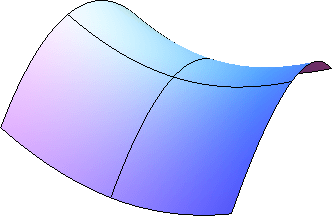
\includegraphics[width=0.4\textwidth]{img/chap4/image046.png}~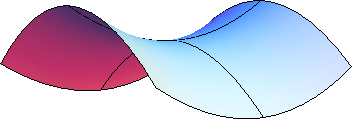
\includegraphics[width=0.4\textwidth]{img/chap4/image047.png}\\
    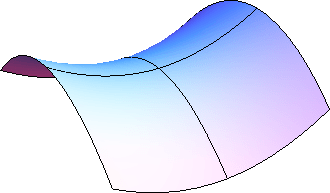
\includegraphics[width=0.4\textwidth]{img/chap4/image048.png}~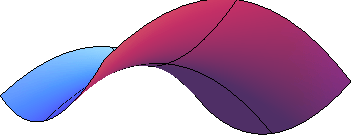
\includegraphics[width=0.4\textwidth]{img/chap4/image049.png}\\
    \caption{Saddle point of $z=f(x,y)=5x^2-3y^2+10$}
    \label{fig:4-3-saddle}
\end{figure}

\subsection{Second Derivative Test}
Just as in the one-variable case, we'll need a way to test a critical point to see whether it is a local maximum or minimum. There is a second derivative test for functions of two variables that can help, but, just as in the one-variable case, it isn't always conclusive.

\begin{theorem}[The Second Derivative Test\index{Second Derivative Test} for Functions of Two Variables]
\label{thm:4-second-deriv-test}
Find all critical points of $f(x,y)$.
Compute
$$D(x,y)=(f_{xx})(f_{yy})-(f_{xy})(f_{yx}) \enspace ,$$
and evaluate $D = D(x,y)$ at each critical point.
  \begin{enumerate}[label = (\alph*)]
    \item If $D>0$, then $f$ has a local maximum or minimum at the critical point. To see which, look at the sign of $f_{xx}$:
    \begin{itemize}
      \item If $f_{xx} > 0$, then $f$ has a local minimum\index{Local minimum} at the critical point.
      \item If $f_{xx} < 0$, then $f$ has a local maximum\index{Local maximum} at the critical point.
    \end{itemize}
    \item If $D<0$ then $f$ has a saddle point at the critical point.
    \item If $D=0$, there could be a local maximum, local minimum or neither (i.e., the test in inconclusive).
  \end{enumerate}
\end{theorem}
\begin{example}
Find all local maxima, minima, and saddle points for the function
$$f(x,y)=x^3+y^3+3x^2-3y^2-8 \enspace.$$

\begin{solution}
  First we find the partial derivatives: $f_x=3x^2+6x$ and $f_y=3y^2-6y$.

Critical points are the places where both of these are zero (neither is ever undefined): $f_x=3x^2+6x=3x(x+2)=0$ when $x=0$ or when $x=-2$. $f_y=3y^2-6y=3y(y-2)=0$ when $y=0$ or when $y=2$.

Putting these together, we get four critical points: $(0, 0)$, $(-2, 0)$, $(0, 2)$, and $(-2, 2)$.

Now to classify them, we'll use Theorem \ref{thm:4-second-deriv-test}, the Second Derivative Test. We'll need all the second partial derivatives:
$$f_{xx}=6x+6 \enspace, \quad f_{yy}=6y-6 \enspace, \quad f_{xy}=f_{yx}=0 \enspace. $$
Then
$$D(x,y)=(6x+6)(6y-6)-(0)(0)=(6x+6)(6y-6) \enspace .$$
Now look at each critical point in turn:
  \begin{itemize}
    \item At $(0, 0)$: $D(0,0)=(6(0)+6)(6(0)-6)=(6)(-6)=-36<0$, so there is a saddle point at the point $(0, 0)$.
    \item At $(-2, 0)$: $D(-2,0)=(6(-2)+6)(6(0)-6)=(-6)(-6)=36>0$ and $f_{xx}(-2,0)=6(-2)+6=-6<0$, so there is a local maximum at the point $(-2, 0)$.
    \item At $(0, 2)$: $D(0,2)=(6(0)+6)(6(2)-6)=(6)(6)=36>0$ and $f_{xx}(0,2)=6(0)+6=6>0$, so there is a local minimum at the point $(0, 2)$.
    \item At $(-2, 2)$: $D(-2,2)=(6(-2)+6)(6(2)-6)=(-6)(6)=-36<0$, so there is another saddle point at the point $(-2, 2)$.
  \end{itemize}
\end{solution}\end{example}

\begin{example}
Find all local maxima, minima, and saddle points for the function
$$z=9x^3 + \frac{y^3}{3}-4xy \enspace .$$

\begin{solution}
  We'll need all the partial derivatives and second partial derivatives, so let's compute them all first:
$$z_x = 27x^2-4y \enspace ,\quad z_y = y^2-4x \enspace, $$
$$z_{xx} = 54x \enspace , \quad z_{xy} = z_{yx} = -4 \enspace , \quad z_{yy} = 2y \enspace.$$
Now to find the critical points, we need both $z_x$ and $z_y$ to be zero (neither is ever undefined), so we need to solve this set of equations simultaneously:
\begin{align*}
z_x = 27x^2 - 4y = 0 \\
z_y =   y^2 - 4x = 0
\end{align*}
Perhaps it's been a while since you solved systems of equations. One solution method is the substitution method -- solve one equation for one variable and substitute into the other equation:
$$\begin{cases}
27x^2 - 4y &= 0 \\
y^2 - 4x &= 0
\end{cases} \rightarrow \mbox{ Solve } y^2 - 4x = 0 \mbox{ for } x = \frac{y^2}{4} \enspace ,$$
then substitute into the other equation:
\begin{align*}
27\left(\frac{y^2}{4}\right)^2 - 4y &= 0\\
\frac{27}{16}y^4 - y &= 0
\end{align*}
Now we have just one equation in one variable to solve. Factoring out a $y$ gives
$$y\left(\frac{27}{16}y^3-1\right) = 0 \enspace ,$$
so $y=0$ or $\dfrac{27}{16}y^3-1=0$, giving $y=\sqrt[3]{\dfrac{1}{27/16}} = \dfrac{\sqrt[3]{4}}{3}$.

Plugging back in to the equation $x = \dfrac{y^2}{4}$ to find $x$ gives us the two critical points: $(0,0)$ and $\left(\frac{4}{9}, \frac{4}{3}\right)$.

Now to test them. First compute
\begin{align*}
D(x,y) &= (f_{xx})(f_{yy})-(f_{xy})(f_{yx}) \\
  &= (54x)(2y)-(-4)(-4) \\
  &= 108xy-16
\end{align*}
Then evaluate D at the two critical points:
  \begin{itemize}
    \item At $(0,0)$: $D(0,0)=-16 < 0$, so there is a saddle point at $(0, 0)$.
    \item At $\left(49, \dfrac{\sqrt[3]{4}}{3}\right)$: $D\left(\dfrac{4}{9}, \dfrac{\sqrt[3]{4}}{3}\right) = 16\left(\sqrt[3]{4} - 1\right) > 0$, and $f_{xx}\left(\dfrac{4}{9}, \dfrac{\sqrt[3]{4}}{3}\right) > 0$, so there is a local minimum at the point $\left(\dfrac{4}{9}, \dfrac{\sqrt[3]{4}}{3}\right)$.
  \end{itemize}
\end{solution}\end{example}

\subsection{Applied Optimization}
\begin{example}
A company makes two products. The demand equations for the two products are given below. $p_1$, $p_2$, $q_1$, and $q_2$ are the prices and quantities for Products 1 and 2.
\begin{align*}
  q_1 &= 200 - 3p_1 - p_2 \\
  q_2 &= 150 - p_1 - 2p_2
\end{align*}
Find the price the company should charge for each product in order to maximize total revenue. What is that maximum revenue?

\begin{solution}
Revenue is still price$\times$quantity. If we're selling two products, the total revenue will be the sum of the revenues from the two products:
\begin{align*}
R(p_1,p_2) &= p_1q_1 + p_2q_2 \\
  &= p_1(200 - 3p_1 - p_2) + p_2(150 - p_1 - 2p_2) \\
  &= 200p_1 - 3p_1^2 - 2p_1p_2 + 150p_2 - 2p_2^2 \enspace .
\end{align*}
This is a function of two variables, the two prices, and we need to optimize it (just as in the previous examples). First we find critical points. The notation here gets a bit hard to look at, but hang in there – this is the same stuff we've done before.
$$R_{p_1} = 200-6p_1-2p_2  \quad \text{and}\quad  R_{p_2}=150-2p_1-4p_2.$$
Solving these simultaneously gives the one critical point $(p_1,p_2)=(25,25)$.
To confirm that this gives maximum revenue, we need to use the Second Derivative Test. Find all the second derivatives:
$$R_{p_1p_2} = -6, R_{p_2p_2} = -4, \quad \text{and}\quad  R_{p_1p_2} = R_{p_2p_1} = -2 \enspace .$$
So $D(25, 25) = (-6)(-4)-(-2)(-2)>0$ and $R_{p_1p_2}(25,25) < 0$, so this really is a local maximum.

Thus, to maximize revenue the company should charge \$25 per unit for both products. This will yield a maximum revenue of \$4375.
\end{solution}\end{example}

